\documentclass[10pt,letterpaper,english,hidelinks]{amsart}

\usepackage{amsmath}
\usepackage{amssymb}
\usepackage{amsthm}
\usepackage{fancyhdr}
\usepackage{graphicx}
\usepackage{pgfplots}
\usepackage{tikz}
\usepackage{datetime2}
\usepackage{natbib}
\usepackage[unicode]{hyperref}
\usepackage{mathtools}
\mathtoolsset{showonlyrefs}

\usetikzlibrary{fadings}
\usetikzlibrary{patterns}
\usetikzlibrary{shadows.blur}
\usetikzlibrary{arrows}
\usetikzlibrary{decorations.markings}
\usetikzlibrary{positioning}
\usetikzlibrary{calc}
\usetikzlibrary{math}

\pgfplotsset{compat=1.16}

\DTMnewdatestyle{mydateformat}{%
  \renewcommand{\DTMdisplaydate}[4]{%
    \number##1\ % year
    \DTMenglishmonthname{##2}\ % Month
    \number##3% day
  }%
  \renewcommand{\DTMDisplaydate}{\DTMdisplaydate}%
}
\DTMsetdatestyle{mydateformat}

% text dimensions
\setlength{\textwidth}{6.5in}
\setlength{\textheight}{9in}

% adjust top margins
\setlength{\topmargin}{0in}
\setlength{\voffset}{-30pt}
\setlength{\headheight}{12pt}

% no room for notes on the side
\setlength{\oddsidemargin}{0in}
\setlength{\evensidemargin}{0in}
\setlength{\marginparwidth}{0in}

% space between paragraphs and lines
\setlength{\parskip}{5pt}
\linespread{1.05} % for final submission
% \linespread{2} % for editing drafts

% Hyphenation
\numberwithin{equation}{section}
\hyphenation{semi-stable}

% Numbering for Theorems, Lemmas, etc.
\theoremstyle{plain}
\newtheorem{theorem}{Theorem}[section]
\newtheorem{corollary}[theorem]{Corollary}
\newtheorem{lemma}[theorem]{Lemma}
\newtheorem{conjecture}[theorem]{Conjecture}
\theoremstyle{definition}
\newtheorem{definition}[theorem]{Definition}
\newtheorem{example}[theorem]{Example}
\newtheorem{remark}[theorem]{Remark}
\numberwithin{equation}{section}

% Header Definitions
\fancyhead[L]{\nouppercase{\rightmark}}
\fancyhead[R]{\nouppercase{\leftmark}}

\pagestyle{fancy}

\newcommand{\cech}{\v{C}ech }
\DeclareMathOperator{\Cech}{\textrm{\v{C}ech}}
\DeclareMathOperator{\Ima}{Im}
\DeclareMathOperator{\Ker}{Ker}
\DeclareMathOperator{\nul}{Null}
\DeclareMathOperator{\boundary}{\partial}
\newcommand*{\Z}{\mathbb{Z}}
\newcommand{\bigslant}[2]{%
  \mathchoice
  {{\raisebox{.2em}{$#1$}\left/\raisebox{-.2em}{$#2$}\right.}}
  {{\raisebox{0em}{$#1$}\left/\raisebox{0em}{$#2$}\right.}}
  {{\raisebox{0em}{$#1$}\left/\raisebox{0em}{$#2$}\right.}}
  {{\raisebox{0em}{$#1$}\left/\raisebox{0em}{$#2$}\right.}}
}
\newcommand{\cross}{\times}
\newcommand{\normalsubgroup}{\triangleleft}
\newcommand{\figref}[1]{[Fig. \ref{#1}]}
\newcommand{\subfigref}[2]{[Fig. \ref{#1}, #2]}
\newcommand{\red}[1]{{\color{red} #1}}
\newcommand{\lightgray}[1]{{\color{lightgray} #1}}


\title[Persistent Homology]{Persistent Homology: Computations and Applications}
\author{Stephen Ermshar}
\address{Department of Mathematics, Walla Walla University, College Place, WA 99324}
\thanks{Advisor: Dr. John Foster}

\date{\DTMDisplaydate{2020}{5}{22}{}} % advisor critique due

\begin{document}

\begin{abstract}
    % 300 word abstract.
    Persistent Homology is a method for understanding a numerical multi dimensional data set by observing certain features of shapes generated by the data.
    These features of interest are holes, and can provide clues for how the data is connected or where data may be missing.
    Homology is the study of these holes, and Persistent Homology is a natural application of this topic to data sets.
    This paper will provide an introduction to Simplicial Homology and how it can be applied to a data set.
\end{abstract}
\maketitle

\section{Introduction}

Persistent homology is a tool for understanding the shape of a data set.
For instance, if a data set is a collection of points in two dimensional space, then it can be graphed in a plane.
We can easily look at the graph and see whether the data clumps together in certain places, or if it forms more interesting shapes, like a loop.
We can graph data in one and three dimensions as well, but with dimensions four and higher we're no longer able to intuitively and visually observe the data directly.

In section \ref{sec:homology} we'll explore Homology, which gives us tools to understand structures analogous to holes in a shape, regardless of the dimension in which the shape is embedded.
When we use Persistent Homology, we'll be converting our data into a form where we can apply tools from homology to understand it.
There are a variety of ways to convert data into a form where homology can be applied, most of which, including the one we'll explore in section \ref{sec:cech-complex}, rely on the choice of a scale parameter.
This scale parameter is used to determine whether points in the data set are related to each other based on the distance between them.
We'll want to understand the structure of the data at multiple scales, so we'll look at its homology along a range of scale parameters.
If a structure revealed by homology persists on a wide range of scales then we can feel more confident that this structure is a good approximation for the shape of the data.
In section \ref{sec:persistent-homology} we'll look at different ways of visualizing a data set's homological structure along a range of scales.

Persistent Homology has been used in a wide variety of fields as a data analysis tool, and has some potential applications outside of data analysis as well.
In section \ref{sec:applications} we'll look at some of these uses, and potentially provide a simple demonstration of an insight that can be gathered using persistent homology.

\section{Homology}\label{sec:homology}

\subsection{Simplicial Homology}\label{sec:simplicial-homology}

To calculate homology on our data we'll first need to convert it into a simplicial complex.
A Simplicial complex is just a collection of sets of points from our dataset. Each of these sets of \(n+1\) points is called an \(n\)-simplex \figref{fig:basic-simplices}.
To keep track of signs later on, we'll give each simplex an orientation which will be denoted by the order in which its points are listed.
We'll arbitrarily choose to list the points in increasing order of the point's label.
The resulting simplicial complex will be a graph-like structure, where pairs of connected points are connected by a line, triples by a triangle, four points by a tetrahedron, and \(n\) points by the \(n\)-dimensional analog of a triangle.

\begin{definition}\label{def:simplicial-complex}
    A \textbf{Simplicial Complex} is a finite collection of finite sets such that every subset of every element in the collection is also an element in the collection. \cite{wagner}
\end{definition}

A simplicial complex has the additional requirement that every subset of every set in the complex is itself a set in the complex. This requirement ensures that if a simplex is in the complex then all of the components that make up that simplex are also in the complex. For instance, if we have a triangle, then we also have all of its edges and vertices.

\begin{figure}
    \tikzset{every picture/.style={line width=0.75pt}} %set default line width to 0.75pt

\begin{tikzpicture}[x=0.75pt,y=0.75pt,yscale=-1,xscale=1]

\coordinate (01) at (77,72);
\coordinate (11) at (147,71);
\coordinate (12) at (179,59.5);
\coordinate (21) at (233.21,91.12);
\coordinate (22) at (276.15,74.49);
\coordinate (23) at (239.92,44.11);
\coordinate (31) at (320,65.5);
\coordinate (32) at (345,30.5);
\coordinate (33) at (369,65.5);
\coordinate (34) at (342,90.5);

% 0 Simplex
\draw   [black, fill=black] (01) circle [radius= 3.35] ;

% 1 Simplex
\draw   [black, fill=black] (11) circle [radius= 3.35] ;
\draw   [black, fill=black] (12) circle [radius= 3.35] ;
\draw   (11) -- (12) ;

% 2 Simplex
\draw   [black, fill=lightgray] (21) -- (22) -- (23) -- cycle   ;
\draw   [black, fill=black] (21) circle [radius= 3.35] ;
\draw   [black, fill=black] (22) circle [radius= 3.35] ;
\draw   [black, fill=black] (23) circle [radius= 3.35] ;

% 3 Simplex
\draw   [black, fill=lightgray] (31) -- (32) -- (34) -- cycle   ;
\draw   [black, fill=gray]      (32) -- (33) -- (34) -- cycle   ;
\draw   [dash pattern={on 4.5pt off 4.5pt}]  (31) -- (33) ;
\draw   [black, fill=black] (31) circle [radius= 3.35] ;
\draw   [black, fill=black] (32) circle [radius= 3.35] ;
\draw   [black, fill=black] (33) circle [radius= 3.35] ;
\draw   [black, fill=black] (34) circle [radius= 3.35] ;

% Straight Arrow
\draw [shift={(163,65.25)}, rotate = 520.23] [fill={rgb, 255:red, 0; green, 0; blue, 0 }  ][line width=0.08]  [draw opacity=0] (8.93,-4.29) -- (0,0) -- (8.93,4.29) -- cycle    ;

% Circle Arrow
\draw  [draw opacity=0] (255.97,69.08) .. controls (255.99,69.3) and (256,69.52) .. (256,69.75) .. controls (256,73.48) and (252.87,76.5) .. (249,76.5) .. controls (245.13,76.5) and (242,73.48) .. (242,69.75) .. controls (242,66.02) and (245.13,63) .. (249,63) .. controls (249.81,63) and (250.59,63.13) .. (251.32,63.38) -- (249,69.75) -- cycle ; \draw   (255.97,69.08) .. controls (255.99,69.3) and (256,69.52) .. (256,69.75) .. controls (256,73.48) and (252.87,76.5) .. (249,76.5) .. controls (245.13,76.5) and (242,73.48) .. (242,69.75) .. controls (242,66.02) and (245.13,63) .. (249,63) .. controls (249.81,63) and (250.59,63.13) .. (251.32,63.38) ;
\draw  [fill={rgb, 255:red, 0; green, 0; blue, 0 }  ,fill opacity=1 ] (253.25,70.52) -- (255.25,65.85) -- (258.47,69.77) ;


% Caption Labels
\draw (78,116)   node   [align=left] {0-simplex};
\draw (166,117)  node   [align=left] {1-simplex};
\draw (256,117)  node   [align=left] {2-simplex};
\draw (347,116)  node   [align=left] {3-simplex};
\draw (78,136)   node   [align=left] {(1)};
\draw (166,137)  node   [align=left] {(1,2)};
\draw (256,137)  node   [align=left] {(1,2,3)};
\draw (347,136)  node   [align=left] {(1,2,3,4)};

% Vertex Labels
\draw (01)+(-10,5)  node   [align=left] {1};
\draw (11)+(-10,5)  node   [align=left] {1};
\draw (12)+(10,5)   node   [align=left] {2};
\draw (21)+(-10,5)  node   [align=left] {1};
\draw (22)+(10,5)   node   [align=left] {2};
\draw (23)+(-10,5)  node   [align=left] {3};
\draw (31)+(-10,5)  node   [align=left] {1};
\draw (32)+(10,0)   node   [align=left] {2};
\draw (33)+(10,5)   node   [align=left] {3};
\draw (34)+(-10,5)  node   [align=left] {4};




\end{tikzpicture}

    \caption{}
    \label{fig:basic-simplices}
\end{figure}

\subsection{The Cech Complex}\label{sec:cech-complex}

There are many ways of constructing simplicial complexes from data, but we'll focus on one of the more intuitive and original methods used, the cech complex.

\begin{definition}\label{def:cech-complex}
    Given a set of points \(P\), and a distance \(r\), let \(B_x(r)\) be the ball with radius \(r\) around the point \(x\). The \textbf{\v{C}ech Complex} is given by
		\begin{align*}
            \textrm{\v{C}ech}(r) := \{ S \subseteq P | \bigcap_{x\in S} B_x(r) \neq \emptyset \}
            .
		\end{align*}
		\cite{wagner}
\end{definition}

% should I explain the cech complex or expect the reader to labor over the definition if they're confused?

The radius \(r\) used in the \v{C}ech Complex is the scale parameter that we'll vary when looking for persistence. One can observe that the \v{C}ech Complex fits the definition of a simplicial complex.
% <!-- Since if balls around points in the set intersect at one scale parameter, then they certainly will when the scale parameter increases. -->
Since if the balls around some points intersect, then the balls around any subset of those points must also intersect.

Given a simplicial complex we can draw it as a graph and observe its homological properties.
Figure \ref{fig:example-cech} demonstrates a simplicial complex with one hole surrounded by the simplices \((2,3)\), \((3,4)\), and \((2,4)\).

\begin{figure}
    \centering
    \begin{minipage}{.5\textwidth}
        \centering
        \tikzset{
pattern size/.store in=\mcSize,
pattern size = 5pt,
pattern thickness/.store in=\mcThickness,
pattern thickness = 0.3pt,
pattern radius/.store in=\mcRadius,
pattern radius = 1pt}
\makeatletter
\pgfutil@ifundefined{pgf@pattern@name@_iy1rqtf17}{
\pgfdeclarepatternformonly[\mcThickness,\mcSize]{_iy1rqtf17}
{\pgfqpoint{0pt}{0pt}}
{\pgfpoint{\mcSize+\mcThickness}{\mcSize+\mcThickness}}
{\pgfpoint{\mcSize}{\mcSize}}
{
\pgfsetcolor{\tikz@pattern@color}
\pgfsetlinewidth{\mcThickness}
\pgfpathmoveto{\pgfqpoint{0pt}{0pt}}
\pgfpathlineto{\pgfpoint{\mcSize+\mcThickness}{\mcSize+\mcThickness}}
\pgfusepath{stroke}
}}
\makeatother
\tikzset{every picture/.style={line width=0.75pt}} %set default line width to 0.75pt

\begin{tikzpicture}[x=0.75pt,y=0.75pt,yscale=-1,xscale=1]
%uncomment if require: \path (0,95); %set diagram left start at 0, and has height of 95

\draw [shift={(163,23.5)}, rotate = 99.21] [color={rgb, 255:red, 165; green, 232; blue, 255}  ][fill={rgb, 255:red, 165; green, 232; blue, 255 }  ][line width=0]      (0, 0) circle [x radius= 20, y radius= 20]   ;
\draw [shift={(135,40)}, rotate = 349.29] [color={rgb, 255:red, 165; green, 232; blue, 255}  ][fill={rgb, 255:red, 165; green, 232; blue, 255 }  ][line width=0]      (0, 0) circle [x radius= 20, y radius= 20]   ;
\draw [shift={(13,61)}, rotate = 312.63] [color={rgb, 255:red, 165; green, 232; blue, 255}  ][fill={rgb, 255:red, 165; green, 232; blue, 255 }  ][line width=0]      (0, 0) circle [x radius= 20, y radius= 20]   ;
\draw [shift={(56,17)}, rotate = 0] [color={rgb, 255:red, 165; green, 232; blue, 255}  ][fill={rgb, 255:red, 165; green, 232; blue, 255 }  ][line width=0]      (0, 0) circle [x radius= 20, y radius= 20]   ;
\draw [shift={(69,54)}, rotate = 329.74] [color={rgb, 255:red, 165; green, 232; blue, 255}  ][fill={rgb, 255:red, 165; green, 232; blue, 255 }  ][line width=0]      (0, 0) circle [x radius= 20, y radius= 20]   ;
\draw [shift={(95,25)}, rotate = 353.99] [color={rgb, 255:red, 165; green, 232; blue, 255}  ][fill={rgb, 255:red, 165; green, 232; blue, 255 }  ][line width=0]      (0, 0) circle [x radius= 20, y radius= 20]   ;
\draw [shift={(95,25)}, rotate = 69.78] [color={rgb, 255:red, 165; green, 232; blue, 255}  ][fill={rgb, 255:red, 165; green, 232; blue, 255 }  ][line width=0]      (0, 0) circle [x radius= 20, y radius= 20]   ;
\draw [shift={(135,40)}, rotate = 314.34] [color={rgb, 255:red, 165; green, 232; blue, 255}  ][fill={rgb, 255:red, 165; green, 232; blue, 255 }  ][line width=0]      (0, 0) circle [x radius= 20, y radius= 20]   ;
\draw [shift={(157,60.5)}, rotate = 31.29] [color={rgb, 255:red, 165; green, 232; blue, 255}  ][fill={rgb, 255:red, 165; green, 232; blue, 255 }  ][line width=0]      (0, 0) circle [x radius= 20, y radius= 20]   ;
\draw [shift={(157,60.5)}, rotate = 349.29] [color={rgb, 255:red, 165; green, 232; blue, 255}  ][fill={rgb, 255:red, 165; green, 232; blue, 255 }  ][line width=0]      (0, 0) circle [x radius= 20, y radius= 20]   ;
\draw [shift={(157,60.5)}, rotate = 99.21] [color={rgb, 255:red, 165; green, 232; blue, 255}  ][fill={rgb, 255:red, 165; green, 232; blue, 255 }  ][line width=0]      (0, 0) circle [x radius= 20, y radius= 20]   ;
\draw [shift={(56,17)}, rotate = 312.63] [color={rgb, 255:red, 165; green, 232; blue, 255}  ][fill={rgb, 255:red, 165; green, 232; blue, 255 }  ][line width=0]      (0, 0) circle [x radius= 20, y radius= 20]   ;
\draw [shift={(95,25)}, rotate = 31.29] [color={rgb, 255:red, 165; green, 232; blue, 255}  ][fill={rgb, 255:red, 165; green, 232; blue, 255 }  ][line width=0]      (0, 0) circle [x radius= 20, y radius= 20]   ;
\draw [shift={(95,25)}, rotate = 0] [color={rgb, 255:red, 165; green, 232; blue, 255}  ][fill={rgb, 255:red, 165; green, 232; blue, 255 }  ][line width=0]      (0, 0) circle [x radius= 20, y radius= 20]   ;
\draw [shift={(69,54)}, rotate = 36.87] [color={rgb, 255:red, 165; green, 232; blue, 255}  ][fill={rgb, 255:red, 165; green, 232; blue, 255 }  ][line width=0]      (0, 0) circle [x radius= 20, y radius= 20]   ;
\draw [shift={(56,17)}, rotate = 36.87] [color={rgb, 255:red, 165; green, 232; blue, 255}  ][fill={rgb, 255:red, 165; green, 232; blue, 255 }  ][line width=0]      (0, 0) circle [x radius= 20, y radius= 20]   ;
\draw [shift={(95,25)}, rotate = 329.74] [color={rgb, 255:red, 165; green, 232; blue, 255}  ][fill={rgb, 255:red, 165; green, 232; blue, 255 }  ][line width=0]      (0, 0) circle [x radius= 20, y radius= 20]   ;
\draw [shift={(163,23.5)}, rotate = 353.99] [color={rgb, 255:red, 165; green, 232; blue, 255}  ][fill={rgb, 255:red, 165; green, 232; blue, 255 }  ][line width=0]      (0, 0) circle [x radius= 20, y radius= 20]   ;
\draw [shift={(135,40)}, rotate = 69.78] [color={rgb, 255:red, 165; green, 232; blue, 255}  ][fill={rgb, 255:red, 165; green, 232; blue, 255 }  ][line width=0]      (0, 0) circle [x radius= 20, y radius= 20]   ;
\draw [shift={(163,23.5)}, rotate = 314.34] [color={rgb, 255:red, 165; green, 232; blue, 255}  ][fill={rgb, 255:red, 165; green, 232; blue, 255 }  ][line width=0]      (0, 0) circle [x radius= 20, y radius= 20]   ;
\draw [shift={(255, 50)}, rotate = 314.34] [color={rgb, 255:red, 165; green, 232; blue, 255}  ][fill={rgb, 255:red, 165; green, 232; blue, 255 }  ][line width=0]      (0, 0) circle [x radius= 20, y radius= 20]   ;

%Straight Lines [id:da20686486428426965] (1-2)
% \draw    (13,61) -- (56,17) ;
\draw [shift={(56,17)}, rotate = 312.63] [color={rgb, 255:red, 0; green, 0; blue, 0 }  ][fill={rgb, 255:red, 0; green, 0; blue, 0 }  ][line width=0.75]      (0, 0) circle [x radius= 3.35, y radius= 3.35]   ;
\draw [shift={(13,61)}, rotate = 312.63] [color={rgb, 255:red, 0; green, 0; blue, 0 }  ][fill={rgb, 255:red, 0; green, 0; blue, 0 }  ][line width=0.75]      (0, 0) circle [x radius= 3.35, y radius= 3.35]   ;
%Straight Lines [id:da9899744043809231] (2-4)
\draw    (56,17) -- (95,25) ;
% \draw [shift={(95,25)}, rotate = 0] [color={rgb, 255:red, 0; green, 0; blue, 0 }  ][fill={rgb, 255:red, 0; green, 0; blue, 0 }  ][line width=0.75]      (0, 0) circle [x radius= 3.35, y radius= 3.35]   ;
% \draw [shift={(56,17)}, rotate = 0] [color={rgb, 255:red, 0; green, 0; blue, 0 }  ][fill={rgb, 255:red, 0; green, 0; blue, 0 }  ][line width=0.75]      (0, 0) circle [x radius= 3.35, y radius= 3.35]   ;
%Straight Lines [id:da4483952202454973] (2-3)
\draw    (56,17) -- (69,54) ;
\draw [shift={(69,54)}, rotate = 36.87] [color={rgb, 255:red, 0; green, 0; blue, 0 }  ][fill={rgb, 255:red, 0; green, 0; blue, 0 }  ][line width=0.75]      (0, 0) circle [x radius= 3.35, y radius= 3.35]   ;
\draw [shift={(56,17)}, rotate = 36.87] [color={rgb, 255:red, 0; green, 0; blue, 0 }  ][fill={rgb, 255:red, 0; green, 0; blue, 0 }  ][line width=0.75]      (0, 0) circle [x radius= 3.35, y radius= 3.35]   ;
%Straight Lines [id:da013663715151336797](3-4)
\draw    (69,54) -- (95,25) ;
\draw [shift={(95,25)}, rotate = 329.74] [color={rgb, 255:red, 0; green, 0; blue, 0 }  ][fill={rgb, 255:red, 0; green, 0; blue, 0 }  ][line width=0.75]      (0, 0) circle [x radius= 3.35, y radius= 3.35]   ;
\draw [shift={(69,54)}, rotate = 329.74] [color={rgb, 255:red, 0; green, 0; blue, 0 }  ][fill={rgb, 255:red, 0; green, 0; blue, 0 }  ][line width=0.75]      (0, 0) circle [x radius= 3.35, y radius= 3.35]   ;
%Straight Lines [id:da6445202628566384](4-7)
% \draw    (95,25) -- (163,23.5) ;
\draw [shift={(163,23.5)}, rotate = 353.99] [color={rgb, 255:red, 0; green, 0; blue, 0 }  ][fill={rgb, 255:red, 0; green, 0; blue, 0 }  ][line width=0.75]      (0, 0) circle [x radius= 3.35, y radius= 3.35]   ;
\draw [shift={(95,25)}, rotate = 353.99] [color={rgb, 255:red, 0; green, 0; blue, 0 }  ][fill={rgb, 255:red, 0; green, 0; blue, 0 }  ][line width=0.75]      (0, 0) circle [x radius= 3.35, y radius= 3.35]   ;
%Straight Lines [id:da3743946516627876] (4-5)
% \draw    (95,25) -- (135,40) ;
\draw [shift={(135,40)}, rotate = 69.78] [color={rgb, 255:red, 0; green, 0; blue, 0 }  ][fill={rgb, 255:red, 0; green, 0; blue, 0 }  ][line width=0.75]      (0, 0) circle [x radius= 3.35, y radius= 3.35]   ;
\draw [shift={(95,25)}, rotate = 69.78] [color={rgb, 255:red, 0; green, 0; blue, 0 }  ][fill={rgb, 255:red, 0; green, 0; blue, 0 }  ][line width=0.75]      (0, 0) circle [x radius= 3.35, y radius= 3.35]   ;
%Straight Lines [id:da2401873796980163] (5-7)
\draw    (135,40) -- (163,23.5) ;
\draw [shift={(163,23.5)}, rotate = 314.34] [color={rgb, 255:red, 0; green, 0; blue, 0 }  ][fill={rgb, 255:red, 0; green, 0; blue, 0 }  ][line width=0.75]      (0, 0) circle [x radius= 3.35, y radius= 3.35]   ;
\draw [shift={(135,40)}, rotate = 314.34] [color={rgb, 255:red, 0; green, 0; blue, 0 }  ][fill={rgb, 255:red, 0; green, 0; blue, 0 }  ][line width=0.75]      (0, 0) circle [x radius= 3.35, y radius= 3.35]   ;
%Straight Lines [id:da08347218855288774] (4-6)
% \draw    (95,25) -- (157,60.5) ;
\draw [shift={(157,60.5)}, rotate = 31.29] [color={rgb, 255:red, 0; green, 0; blue, 0 }  ][fill={rgb, 255:red, 0; green, 0; blue, 0 }  ][line width=0.75]      (0, 0) circle [x radius= 3.35, y radius= 3.35]   ;
\draw [shift={(95,25)}, rotate = 31.29] [color={rgb, 255:red, 0; green, 0; blue, 0 }  ][fill={rgb, 255:red, 0; green, 0; blue, 0 }  ][line width=0.75]      (0, 0) circle [x radius= 3.35, y radius= 3.35]   ;
%Straight Lines [id:da34695654406224863]
\draw    (135,40) -- (157,60.5) ;
\draw [shift={(157,60.5)}, rotate = 349.29] [color={rgb, 255:red, 0; green, 0; blue, 0 }  ][fill={rgb, 255:red, 0; green, 0; blue, 0 }  ][line width=0.75]      (0, 0) circle [x radius= 3.35, y radius= 3.35]   ;
\draw [shift={(135,40)}, rotate = 349.29] [color={rgb, 255:red, 0; green, 0; blue, 0 }  ][fill={rgb, 255:red, 0; green, 0; blue, 0 }  ][line width=0.75]      (0, 0) circle [x radius= 3.35, y radius= 3.35]   ;
%Straight Lines [id:da5097015872445443]
\draw    (163,23.5) -- (157,60.5) ;
\draw [shift={(157,60.5)}, rotate = 99.21] [color={rgb, 255:red, 0; green, 0; blue, 0 }  ][fill={rgb, 255:red, 0; green, 0; blue, 0 }  ][line width=0.75]      (0, 0) circle [x radius= 3.35, y radius= 3.35]   ;
\draw [shift={(163,23.5)}, rotate = 99.21] [color={rgb, 255:red, 0; green, 0; blue, 0 }  ][fill={rgb, 255:red, 0; green, 0; blue, 0 }  ][line width=0.75]      (0, 0) circle [x radius= 3.35, y radius= 3.35]   ;

\draw [pattern=_iy1rqtf17,pattern size=6pt,pattern thickness=0.75pt,pattern radius=0pt, pattern color={rgb, 255:red, 0; green, 0; blue, 0}] (135,40) -- (163,23.5) -- (157,60.5) -- cycle ;

% Text Node
\draw (27.5,66.5) node    {$1$};
% Text Node
\draw (65,10) node    {$2$};
% Text Node
\draw (80,58.5) node    {$3$};
% Text Node
\draw (105,16) node    {$4$};
% Text Node
\draw (130,50) node    {$5$};
% Text Node
\draw (172,62) node    {$6$};
% Text Node
\draw (176,13.5) node    {$7$};
% Text Node
\draw[fill={rgb, 255:red, 0; green, 0; blue, 0 }] (255, 50) circle [x radius= 3.35, y radius= 3.35]    (260,40) node    {$8$};



\end{tikzpicture}

    \end{minipage}%
    \begin{minipage}{.5\textwidth}
        \begin{align*}
            C_1 &= \langle (1,2),(1,3),(2,3),(2,4),(3,4) \rangle \\
            C_2 &= \langle (1,2,3) \rangle \\
            \ell_1 &= (2,3) - (1,3) + (1,2) \\
            \ell_0 &= (1,3) + (3,4) - (2,4) - (1,2)
        \end{align*}
    \end{minipage}
    \caption{}
    \label{fig:example-cech}
\end{figure}

\subsection{Computations}

\section{Persistent Homology}\label{sec:persistent-homology}

\subsection{Persistence Barcodes}

\subsection{Persistence Diagrams}

\section{Applications}\label{sec:applications}

\newpage

\bibliographystyle{alpha}
\bibliography{../math496-7-zotero.bib}

\end{document}
